% Options for packages loaded elsewhere
\PassOptionsToPackage{unicode}{hyperref}
\PassOptionsToPackage{hyphens}{url}
%
\documentclass[
]{article}
\usepackage{amsmath,amssymb}
\usepackage{iftex}
\ifPDFTeX
  \usepackage[T1]{fontenc}
  \usepackage[utf8]{inputenc}
  \usepackage{textcomp} % provide euro and other symbols
\else % if luatex or xetex
  \usepackage{unicode-math} % this also loads fontspec
  \defaultfontfeatures{Scale=MatchLowercase}
  \defaultfontfeatures[\rmfamily]{Ligatures=TeX,Scale=1}
\fi
\usepackage{lmodern}
\ifPDFTeX\else
  % xetex/luatex font selection
\fi
% Use upquote if available, for straight quotes in verbatim environments
\IfFileExists{upquote.sty}{\usepackage{upquote}}{}
\IfFileExists{microtype.sty}{% use microtype if available
  \usepackage[]{microtype}
  \UseMicrotypeSet[protrusion]{basicmath} % disable protrusion for tt fonts
}{}
\makeatletter
\@ifundefined{KOMAClassName}{% if non-KOMA class
  \IfFileExists{parskip.sty}{%
    \usepackage{parskip}
  }{% else
    \setlength{\parindent}{0pt}
    \setlength{\parskip}{6pt plus 2pt minus 1pt}}
}{% if KOMA class
  \KOMAoptions{parskip=half}}
\makeatother
\usepackage{xcolor}
\usepackage[margin=1in]{geometry}
\usepackage{color}
\usepackage{fancyvrb}
\newcommand{\VerbBar}{|}
\newcommand{\VERB}{\Verb[commandchars=\\\{\}]}
\DefineVerbatimEnvironment{Highlighting}{Verbatim}{commandchars=\\\{\}}
% Add ',fontsize=\small' for more characters per line
\usepackage{framed}
\definecolor{shadecolor}{RGB}{248,248,248}
\newenvironment{Shaded}{\begin{snugshade}}{\end{snugshade}}
\newcommand{\AlertTok}[1]{\textcolor[rgb]{0.94,0.16,0.16}{#1}}
\newcommand{\AnnotationTok}[1]{\textcolor[rgb]{0.56,0.35,0.01}{\textbf{\textit{#1}}}}
\newcommand{\AttributeTok}[1]{\textcolor[rgb]{0.13,0.29,0.53}{#1}}
\newcommand{\BaseNTok}[1]{\textcolor[rgb]{0.00,0.00,0.81}{#1}}
\newcommand{\BuiltInTok}[1]{#1}
\newcommand{\CharTok}[1]{\textcolor[rgb]{0.31,0.60,0.02}{#1}}
\newcommand{\CommentTok}[1]{\textcolor[rgb]{0.56,0.35,0.01}{\textit{#1}}}
\newcommand{\CommentVarTok}[1]{\textcolor[rgb]{0.56,0.35,0.01}{\textbf{\textit{#1}}}}
\newcommand{\ConstantTok}[1]{\textcolor[rgb]{0.56,0.35,0.01}{#1}}
\newcommand{\ControlFlowTok}[1]{\textcolor[rgb]{0.13,0.29,0.53}{\textbf{#1}}}
\newcommand{\DataTypeTok}[1]{\textcolor[rgb]{0.13,0.29,0.53}{#1}}
\newcommand{\DecValTok}[1]{\textcolor[rgb]{0.00,0.00,0.81}{#1}}
\newcommand{\DocumentationTok}[1]{\textcolor[rgb]{0.56,0.35,0.01}{\textbf{\textit{#1}}}}
\newcommand{\ErrorTok}[1]{\textcolor[rgb]{0.64,0.00,0.00}{\textbf{#1}}}
\newcommand{\ExtensionTok}[1]{#1}
\newcommand{\FloatTok}[1]{\textcolor[rgb]{0.00,0.00,0.81}{#1}}
\newcommand{\FunctionTok}[1]{\textcolor[rgb]{0.13,0.29,0.53}{\textbf{#1}}}
\newcommand{\ImportTok}[1]{#1}
\newcommand{\InformationTok}[1]{\textcolor[rgb]{0.56,0.35,0.01}{\textbf{\textit{#1}}}}
\newcommand{\KeywordTok}[1]{\textcolor[rgb]{0.13,0.29,0.53}{\textbf{#1}}}
\newcommand{\NormalTok}[1]{#1}
\newcommand{\OperatorTok}[1]{\textcolor[rgb]{0.81,0.36,0.00}{\textbf{#1}}}
\newcommand{\OtherTok}[1]{\textcolor[rgb]{0.56,0.35,0.01}{#1}}
\newcommand{\PreprocessorTok}[1]{\textcolor[rgb]{0.56,0.35,0.01}{\textit{#1}}}
\newcommand{\RegionMarkerTok}[1]{#1}
\newcommand{\SpecialCharTok}[1]{\textcolor[rgb]{0.81,0.36,0.00}{\textbf{#1}}}
\newcommand{\SpecialStringTok}[1]{\textcolor[rgb]{0.31,0.60,0.02}{#1}}
\newcommand{\StringTok}[1]{\textcolor[rgb]{0.31,0.60,0.02}{#1}}
\newcommand{\VariableTok}[1]{\textcolor[rgb]{0.00,0.00,0.00}{#1}}
\newcommand{\VerbatimStringTok}[1]{\textcolor[rgb]{0.31,0.60,0.02}{#1}}
\newcommand{\WarningTok}[1]{\textcolor[rgb]{0.56,0.35,0.01}{\textbf{\textit{#1}}}}
\usepackage{longtable,booktabs,array}
\usepackage{calc} % for calculating minipage widths
% Correct order of tables after \paragraph or \subparagraph
\usepackage{etoolbox}
\makeatletter
\patchcmd\longtable{\par}{\if@noskipsec\mbox{}\fi\par}{}{}
\makeatother
% Allow footnotes in longtable head/foot
\IfFileExists{footnotehyper.sty}{\usepackage{footnotehyper}}{\usepackage{footnote}}
\makesavenoteenv{longtable}
\usepackage{graphicx}
\makeatletter
\def\maxwidth{\ifdim\Gin@nat@width>\linewidth\linewidth\else\Gin@nat@width\fi}
\def\maxheight{\ifdim\Gin@nat@height>\textheight\textheight\else\Gin@nat@height\fi}
\makeatother
% Scale images if necessary, so that they will not overflow the page
% margins by default, and it is still possible to overwrite the defaults
% using explicit options in \includegraphics[width, height, ...]{}
\setkeys{Gin}{width=\maxwidth,height=\maxheight,keepaspectratio}
% Set default figure placement to htbp
\makeatletter
\def\fps@figure{htbp}
\makeatother
\setlength{\emergencystretch}{3em} % prevent overfull lines
\providecommand{\tightlist}{%
  \setlength{\itemsep}{0pt}\setlength{\parskip}{0pt}}
\setcounter{secnumdepth}{-\maxdimen} % remove section numbering
\ifLuaTeX
  \usepackage{selnolig}  % disable illegal ligatures
\fi
\usepackage{bookmark}
\IfFileExists{xurl.sty}{\usepackage{xurl}}{} % add URL line breaks if available
\urlstyle{same}
\hypersetup{
  pdftitle={Online Shoppers Intention},
  pdfauthor={Giuseppe Leonardi, Barbara Micalizzi, Gaetano De Angelis, Rosario Pavone},
  hidelinks,
  pdfcreator={LaTeX via pandoc}}

\title{Online Shoppers Intention}
\author{Giuseppe Leonardi, Barbara Micalizzi, Gaetano De Angelis,
Rosario Pavone}
\date{}

\begin{document}
\maketitle

{
\setcounter{tocdepth}{4}
\tableofcontents
}
\newpage

\section{Introduction}\label{introduction}

The purpose of this report is to outline the training procedure for a
data-set aimed at predicting future values of a specific variable. We
will utilize the ``Online Shoppers Intention'' data-set, with
approximately 80\% of its units allocated to the training set and the
remaining 20\% to the test set. Our focal variable is ``Revenue,'' which
is absent from the test set. Hence, our objective is to forecast future
revenue values, thereby predicting, based on user behavior, whether a
given user is likely to make a purchase.

The data-set encompasses feature vectors for 12,330 sessions, each
representing a distinct user across a one-year time-frame. It has been
meticulously curated to mitigate bias towards particular campaigns,
special occasions, user profiles, or time periods.

The 18 features of the data-set are the following:

\textbf{Administrative}: The number of pages of this type
(administrative) visited by the user in that session.

\textbf{Administrative\_Duration}: The total amount of time (in seconds)
spent by the user on administrative pages during the session.

\textbf{Informational}: The number of informational pages visited by the
user in that session.

\textbf{Informational\_Duration}: The total time spent by the user on
informational pages.

\textbf{ProductRelated}: The number of product-related pages visited by
the user.

\textbf{ProductRelated\_Duration}: The total time spent by the user on
product-related pages.

\textbf{BounceRates}: The average bounce rate of the pages visited by
the user. The bounce rate is the percentage of visitors who navigate
away from the site after viewing only one page.

\textbf{ExitRates}: The average exit rate of the pages visited by the
user. The exit rate is a metric that shows the percentage of exits from
a page.

\textbf{PageValues}: The average value of the pages visited by the user.
This metric is often used as an indicator of how valuable a page is in
terms of generating revenue.

\textbf{SpecialDay}: This indicates the closeness of the site visiting
time to a specific special day (e.g., Mother's Day, Valentine's Day) in
which the sessions are more likely to be finalized with a transaction.

\textbf{Month}: The month of the year in which the session occurred.

\textbf{OperatingSystems}: The operating system used by the user.

\textbf{Browser}: The browser used by the user.

\textbf{Region}: The region from which the user is accessing the
website.

\textbf{TrafficType}: Refers to the source from which visitor come to a
website (e.g.~direct, paid search, organic search, referral).

\textbf{VisitorType}: A categorization of users (e.g., Returning
Visitor, New Visitor).

\textbf{Weekend}: A Boolean indicating whether the session occurred on a
weekend.

\textbf{Revenue}: A binary variable indicating whether the session ended
in a transaction (purchase).

The variables type are:

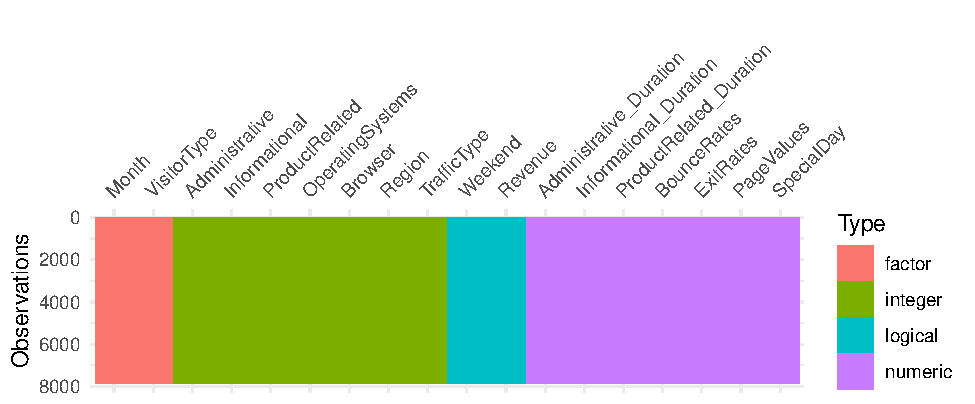
\includegraphics{report_official_files/figure-latex/unnamed-chunk-2-1.pdf}

So, looking at the plot above, we observe that there are no missing
values and the variables are categorized as follows:

\begin{itemize}
\item
  seven integer variables;
\item
  seven float variables;
\item
  two logical variables;
\item
  two categorical variables;
\end{itemize}

The variables \texttt{OperatingSystems}, \texttt{Browser},
\texttt{Region},\texttt{TrafficType} and \texttt{SpecialDay} are
classified as integer, but all of this variables are in fact
categorical, so \emph{we decide to transform the already mentioned them}
(see the appendix for the code).

The data-set includes various features about user behavior on a website,
such as the number of pages visited in different categories
(administrative, informational, product-related) and the duration spent
on these pages. There are also features regarding the technical aspects
of the visit (operating system, browser, region, traffic type) and some
temporal aspects (month, special day, weekend).

The final column, `\textbf{\texttt{Revenue}}', that will be our
dependent variable, is a Boolean indicating whether the visit led to a
purchase, making this data-set potentially useful for predictive
modeling in e-commerce analytics.

\section{Question for the Analysis}\label{question-for-the-analysis}

\begin{enumerate}
\def\labelenumi{\arabic{enumi}.}
\item
  What are the visitor characteristics that most influence the
  probability of generating revenue? Is there a relationship between
  visitor behavior (e.g., bounce rate, exit rate) and revenue
  generation?
\item
  Are there certain days of the week or months of the year more
  favorable for revenue generation? Do demographic or geographic
  characteristics of visitors influence the probability of revenue
  generation?
\item
  Are there differences in behavior between new and returning visitors?
  How do visitor technical characteristics influence the probability of
  revenue generation?
\end{enumerate}

\newpage

\section{Exploratory Data Analysis}\label{exploratory-data-analysis}

Let's start the analysis with a focus on the principal measures for the
numerical variables:

\begin{longtable}[]{@{}
  >{\raggedleft\arraybackslash}p{(\columnwidth - 10\tabcolsep) * \real{0.3788}}
  >{\centering\arraybackslash}p{(\columnwidth - 10\tabcolsep) * \real{0.1364}}
  >{\centering\arraybackslash}p{(\columnwidth - 10\tabcolsep) * \real{0.1364}}
  >{\centering\arraybackslash}p{(\columnwidth - 10\tabcolsep) * \real{0.0909}}
  >{\centering\arraybackslash}p{(\columnwidth - 10\tabcolsep) * \real{0.1515}}
  >{\centering\arraybackslash}p{(\columnwidth - 10\tabcolsep) * \real{0.1061}}@{}}
\toprule\noalign{}
\begin{minipage}[b]{\linewidth}\raggedleft
\end{minipage} & \begin{minipage}[b]{\linewidth}\centering
mean
\end{minipage} & \begin{minipage}[b]{\linewidth}\centering
sd
\end{minipage} & \begin{minipage}[b]{\linewidth}\centering
skew
\end{minipage} & \begin{minipage}[b]{\linewidth}\centering
kurtosis
\end{minipage} & \begin{minipage}[b]{\linewidth}\centering
se
\end{minipage} \\
\midrule\noalign{}
\endhead
\bottomrule\noalign{}
\endlastfoot
Administrative & 2.32 & 3.34 & 1.96 & 4.73 & 0.04 \\
Administrative\_Duration & 80.48 & 175.51 & 5.58 & 50.09 & 1.98 \\
Informational & 0.50 & 1.25 & 3.58 & 17.30 & 0.01 \\
Informational\_Duration & 34.13 & 137.16 & 7.46 & 75.42 & 1.54 \\
ProductRelated & 31.88 & 45.15 & 4.39 & 31.46 & 0.51 \\
ProductRelated\_Duration & 1191.49 & 1944.29 & 7.89 & 162.78 & 21.89 \\
BounceRates & 0.02 & 0.05 & 2.92 & 7.49 & 0.00 \\
ExitRates & 0.04 & 0.05 & 2.12 & 3.87 & 0.00 \\
PageValues & 5.92 & 18.84 & 6.57 & 70.48 & 0.21 \\
\end{longtable}

Each variable presents different measures, except for
\texttt{BounceRates} and \texttt{ExitRate}, which can be considered
quite similar in terms of both mean and standard deviation.

Variables related to the time spent on a page (\texttt{\%\%\_Duration})
indicate that, on average, the users spent more time on pages of similar
products. However, this observation is more subjective due to the
variability indicated by the standard deviation. Conversely, other
variables suggest less time spent on average on such pages, but with a
lower standard deviation, implying that users spend roughly the same
amount of time on pages of this type.

For the same reasons, variables expressing the number of pages of one
type visited by a user show higher values for pages of similar products
and less values on page of Administration and Informational.

the high Kurtosis for each variable (some so much more than others)
indicates that there are more data points concentrated in the central
part of the distribution and fewer data points in the tails. Heavier
tails may indicate the presence of outliers, which are extreme values
that deviate significantly from the mean.

\newpage

\subsection{Visualization}\label{visualization}

The analysis of the categorical variables give us some suggestion:

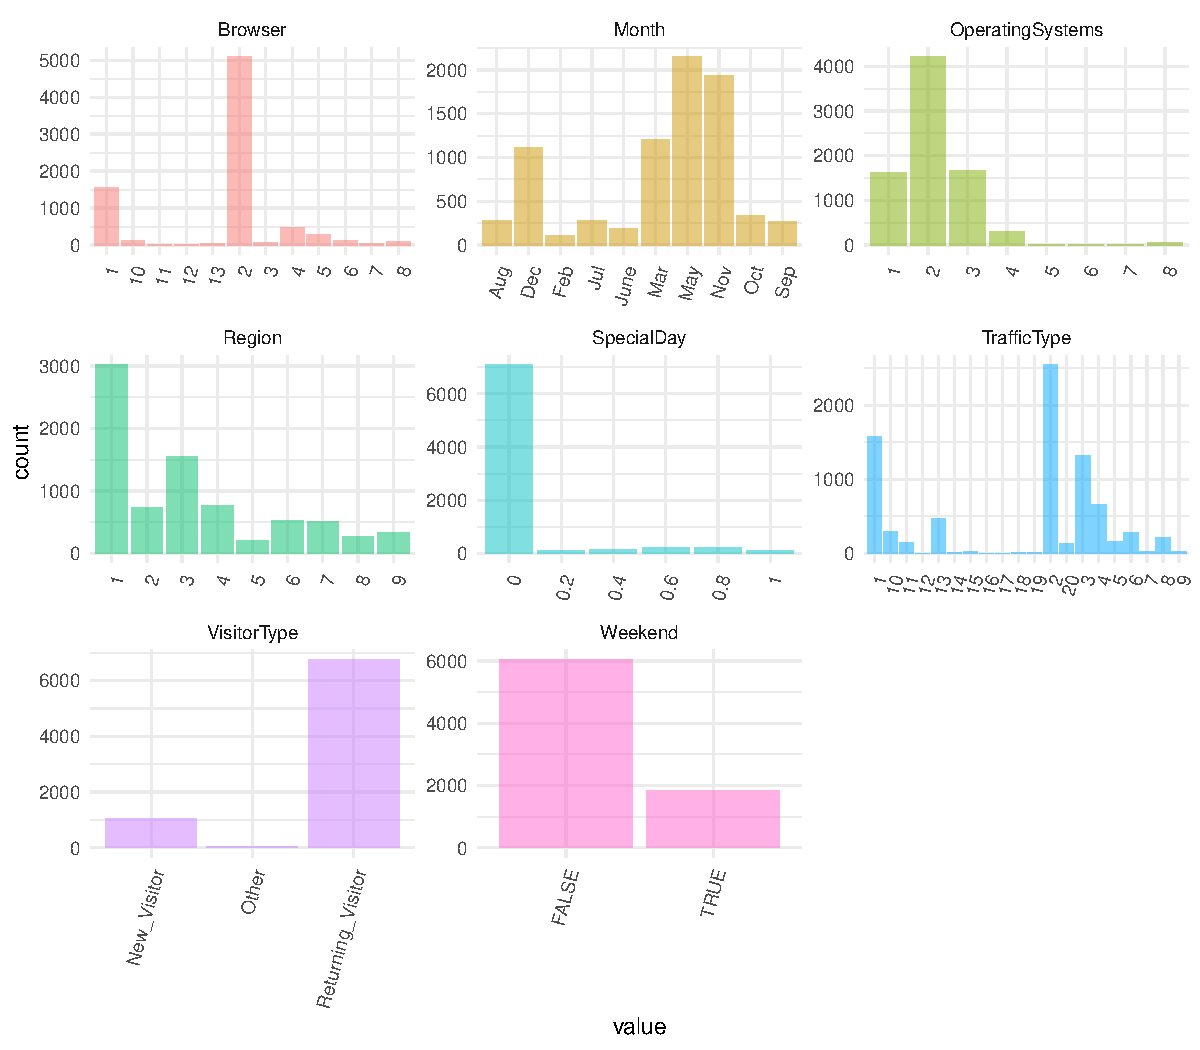
\includegraphics{report_official_files/figure-latex/unnamed-chunk-5-1.pdf}

we note that:

\begin{itemize}
\item
  For the variable \texttt{Months}, we see that \texttt{May},
  \texttt{November}, and \texttt{March} are the months with the highest
  sales, while January and April are absent in the records. We are not
  sure of the reasons for this absence, but we assume it could be due to
  either no registrations or perhaps they were not relevant in terms of
  sales.
\item
  For the variables \texttt{Browser} and \texttt{Operating\ System}, we
  notice that there is one type more commonly used than the others
  (number \texttt{2}). This could be justified by the fact that the
  majority of users are Android smartphone users with Chrome browser
  installed. Therefore, it is deduced that this difference may be due to
  this.
\item
  for the variable \texttt{Special\ Day} when the value is 1 means that
  we are close to a holiday, while when the value is 0, the visit
  session was not conducted near a Special Day. As we can observe, most
  of the search sessions are conducted far from Special days.
\end{itemize}

As we can see from the density plots belove, \emph{the features of our
data set don't meet the \textbf{normality assumption}.}

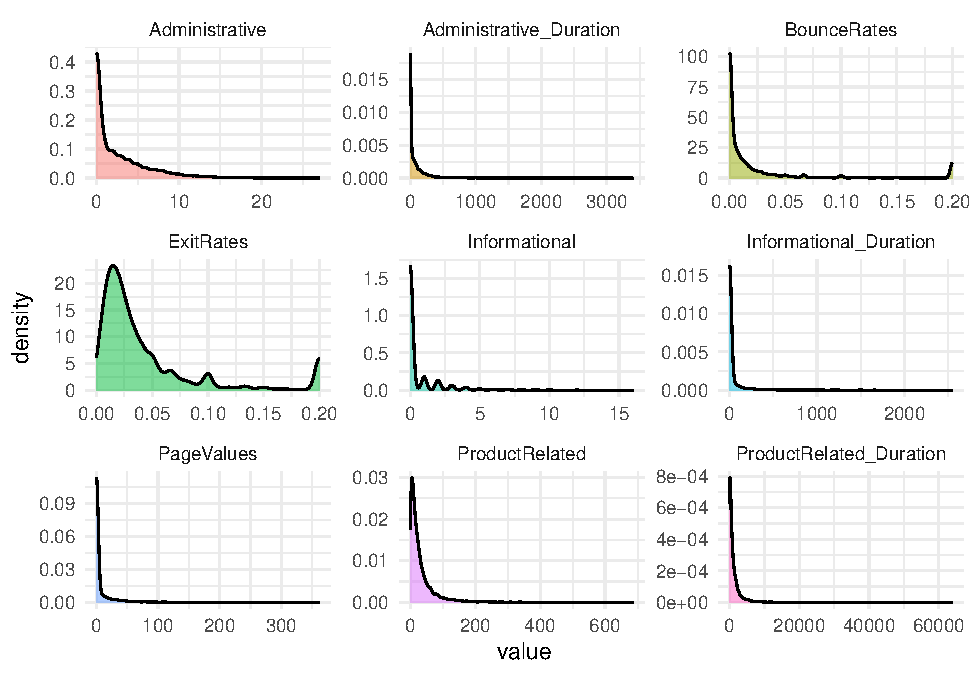
\includegraphics{report_official_files/figure-latex/unnamed-chunk-6-1.pdf}

all this data presents a \textbf{\emph{right-skewed distribution.}} It
is evident that exitRates exhibit significant variability, as all its
values repeat more or less frequently, also concentrating around values
close to zero. A similar pattern can be observed for BounceRates. All
other variables show minimal fluctuations, with very few outliers.

\subsection{Correlation}\label{correlation}

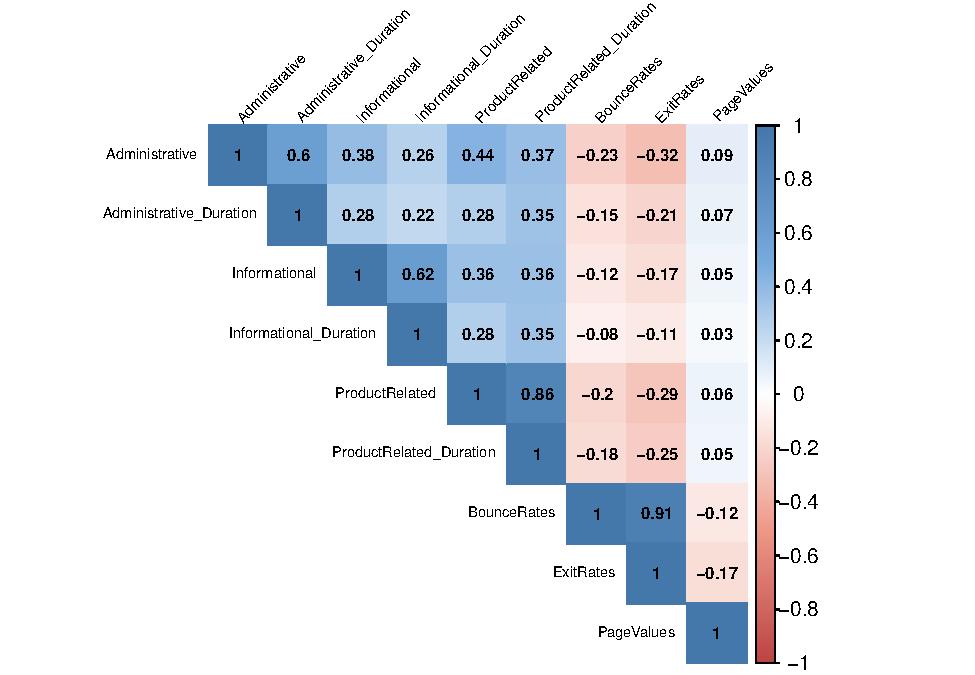
\includegraphics{report_official_files/figure-latex/unnamed-chunk-7-1.pdf}

The variables with high correlation are:

\begin{itemize}
\item
  \texttt{BounceRates} and \texttt{ExitRates}, with a positive
  correlation of 0.91, and it is obvious because they are both
  considering the exit-rate of a page;
\item
  \texttt{ProductRelated} and \texttt{ProductRelated\_Duration} (0.86),
  and this make sense, because more pages visited of the related
  products, more time spent on pages of this type;
\item
  \texttt{Administrative}/\texttt{AdministrativeDuration} (0.60) and
  \texttt{Informational}/\texttt{InformationalDuration} (0.63), for the
  same reason of the other couple of predictors;
\end{itemize}

All of the variables mentioned above, are correlated between them, but
with a small positive value (from 0.20 to 0.40). The low positive
correlation suggests that website visitors engage in diverse and
comprehensive exploration of the site's content during a shopping
session, rather than focusing solely on one type of page. A variety of
visited pages may also reflect effective website design that guides
users through an intuitive and informative path during the shopping
process.

We can also see that the there's a negative (but not strong) correlation
between the variables \texttt{BounceRate} and \texttt{ExitRate} with the
other predictors, and this is due to the fact that if you go away from a
page or from the site, you will never see the other page of the site.

\newpage

\subsection{Target Variable}\label{target-variable}

\texttt{Revenue} can assume two value:

\begin{itemize}
\item
  \textbf{False}, if the session of shopping doesn't end with a
  purchase;
\item
  \textbf{True}, when the session ends with a purchase.
\end{itemize}

\begin{verbatim}
## Revenue
## FALSE  TRUE 
##  6668  1222
\end{verbatim}

Most of the time, the session will end without a purchase.

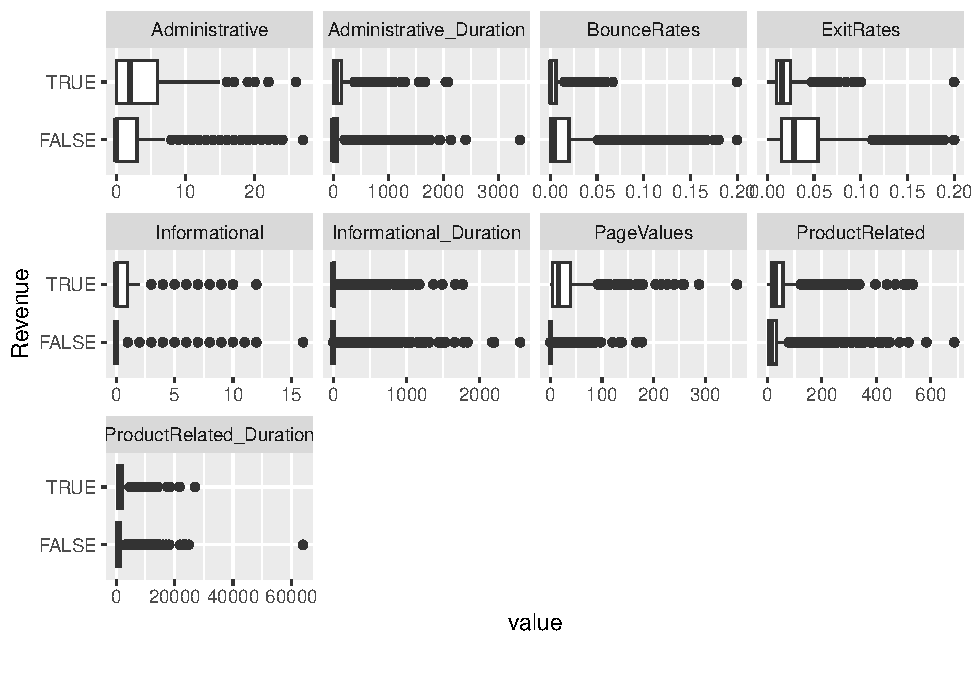
\includegraphics{report_official_files/figure-latex/unnamed-chunk-9-1.pdf}

As expected, the plots that explain the values connected to the pages
(\texttt{Administrative}, \texttt{Informational} and so on) have greater
value in the class TRUE, so the users that spent more time on the page
of a website, maybe can have a greatest probability to do a purchase
online than who doesn't.

Conversely, the value of \texttt{BounceRates} and \texttt{ExitRates} are
greater in the class FALSE (as expected, because if you go out from a
page it's unlikely you to do a purchase).

\newpage

\section{Classification}\label{classification}

First of all, considering the amount of feauters in our data set, we
consider to reduce the number of variables that will be useful to
predict our target variable. after some analisys based on the value of
the AIC (see the appendix for the complete procedure), we choose the
following model, that have the smallest AIC:

\begin{verbatim}
Call:
glm(formula = Revenue ~ Informational + ProductRelated_Duration + 
    BounceRates + ExitRates + PageValues + Month + VisitorType + 
    Weekend, family = "binomial", data = dt_train)
\end{verbatim}

So, the next step is to fit a model on this features and see the
goodness of fit of that.

\subsection{Logistic Regression}\label{logistic-regression}

fitting a logistic regression on the data set specified above, we obtain
the following results:

\begin{verbatim}
    Null deviance: 6802.5  on 7889  degrees of freedom
Residual deviance: 4518.2  on 7872  degrees of freedom
AIC: 4554.2

Number of Fisher Scoring iterations: 7
\end{verbatim}

Giving a look at the summary of the model (in the appendix), we see
that:

\begin{itemize}
\item
  \texttt{Informational}, \texttt{ProductRelated\_Duration},
  \texttt{ExitRates}, and \texttt{PageValues} and others have
  statistically significant coefficients, implying that they are
  associated with the probability of a purchase.
\item
  \emph{Categorical} \emph{variables} such as \texttt{Month},
  \texttt{VisitorType}, and \texttt{TrafficType} have levels that are
  significantly associated with the probability of a purchase, as
  indicated by their coefficients.
\item
  The significant decrease of the variance between \emph{Null} and
  \emph{Residual} explain that the model which consider all the
  variables in the model is better in order to make predictions.
\item
  The model required 12 iterations of the Fisher Scoring algorithm to
  converge to the final parameter estimates, that in fact is a good
  results;
\end{itemize}

\begin{verbatim}
          Actual
Predicted FALSE TRUE
    FALSE  1628  195
    TRUE     41  109

     Accuracy Precision Recall F1-Score
[1,]   0.8804    0.7267 0.3586   0.4802
\end{verbatim}

\begin{itemize}
\item
  \textbf{Accuracy}: 88\% of the predictions made by the model were
  correct. It's a measure of overall model performance.
\item
  \textbf{Precision}: when the model predicts a positive class (TRUE),
  it is correct approximately 72\% of the time. It's a measure of the
  correctness of positive predictions.
\item
  \textbf{Recall}: suggests that the model correctly identifies about
  36\% of the actual positive cases. It's a measure of the completeness
  of positive predictions.
\item
  \textbf{F1-Score}: An F1-score reaches its best value at 1 and worst
  at 0, so we reached a medium result.
\end{itemize}

Overall, the model seems to have decent performance. We try to see if
with a lasso selection of the variables we can obtain better results.

\begin{verbatim}
Call:
glm(formula = Revenue ~ ProductRelated + ProductRelated_Duration + 
    ExitRates + PageValues, family = "binomial", data = dt_train)

    Null deviance: 6802.5  on 7889  degrees of freedom
Residual deviance: 4701.6  on 7885  degrees of freedom
AIC: 4711.6

Number of Fisher Scoring iterations: 7
\end{verbatim}

the AIC and the variance show that the two models are so similar. We
repeat the procedure of predictions, to see the behavior of this new
model.

\begin{verbatim}
          Actual
Predicted FALSE TRUE
    FALSE  1631  197
    TRUE     38  107

     Accuracy Precision Recall F1-Score
[1,]   0.8809    0.7379  0.352   0.4766
\end{verbatim}

The model trained with LASSO selection achieved results that were only
slightly better than the initial model. We decided to use this model
because it is also simpler to implement. But now, we implement our
analysis with a LDA \& QDA.

\subsection{LDA}\label{lda}

Our rationale for selecting the same set of variables as logistic
regression is twofold. Firstly, these variables have exhibited
significant associations in our prior analysis. Secondly, by maintaining
consistency in variable selection, we aim to establish a coherent
analytical framework, facilitating seamless comparison and
interpretation of results between the two methodologies.

\begin{verbatim}
Call:
lda(Revenue ~ ProductRelated + ProductRelated_Duration + ExitRates + 
    PageValues, data = dt_train)

Prior probabilities of groups:
    FALSE      TRUE 
0.8451204 0.1548796 
\end{verbatim}

As we can see the prior probability of the class FALSE it's so much
higher than the other class. to understand if this model it's better
then the logistic regression model, we can use the same statistical
index, starting from the confusion matrix.

\newpage

\begin{verbatim}
          Actual
Predicted FALSE TRUE
    FALSE  1637  211
    TRUE     32   93

     Accuracy Precision Recall F1-Score
[1,]   0.8768     0.744 0.3059   0.4336
\end{verbatim}

in this case, we obtained similar result of the logistic regression.

\subsection{QDA}\label{qda}

For the similar reasons specified for the LDA, we used the same features
as before, with the following results:

\begin{verbatim}
Call:
qda(Revenue ~ ProductRelated + ProductRelated_Duration + ExitRates + 
    PageValues, data = dt_train)

Prior probabilities of groups:
    FALSE      TRUE 
0.8451204 0.1548796 
\end{verbatim}

\begin{verbatim}
          Actual
Predicted FALSE TRUE
    FALSE  1586  163
    TRUE     83  141

     Accuracy Precision Recall F1-Score
[1,]   0.8753    0.6295 0.4638   0.5341
\end{verbatim}

Comparing the metrics for all four models obtained, we notice that the
differences are truly minimal. To confidently determine which model to
use in this case, we can resort to the ROC curve and AUC (Area Under the
Curve).

\newpage

\subsection{ROC curve}\label{roc-curve}

Calculating the ROC curves and the Area Under the Curve (AUC) for the
validation set of each of the four models analyzed, we observe that all
four achieve rather similar results, with a slightly higher AUC value
for the model trained with QDA.

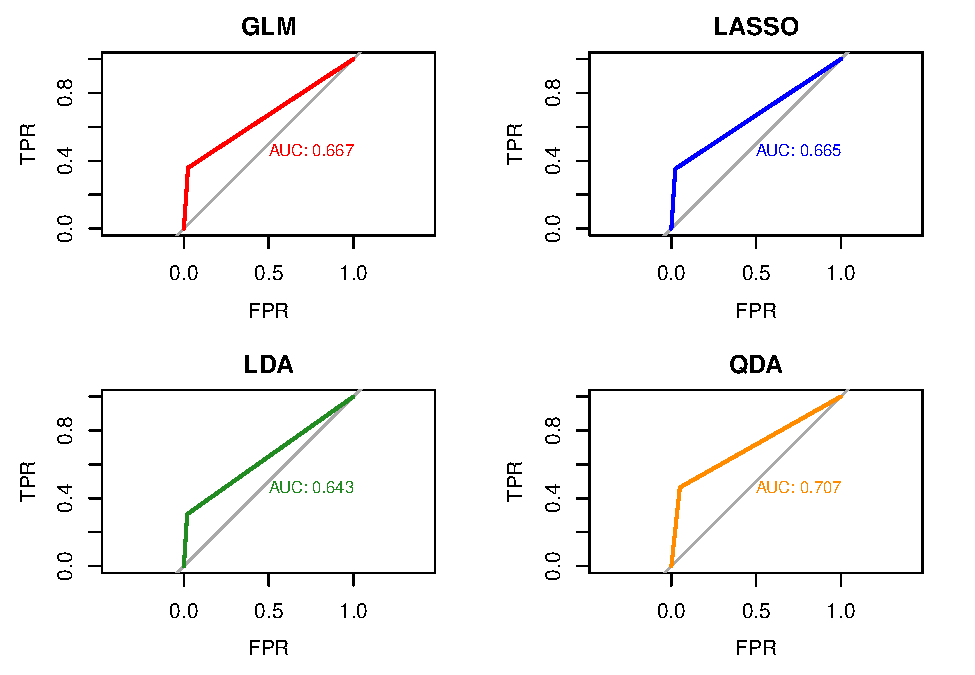
\includegraphics{report_official_files/figure-latex/unnamed-chunk-19-1.pdf}

to do our predictions on the test set, we decide to use the the logistic
regression model trained with the features choosed by the step-analysis
(predictions in the appendix), and with the QDA model (that obatain
better results in term of confusion matrix and AUC).

\newpage

\section{Predictions}\label{predictions}

In order to complete our analysis, the final step is to apply the
choosen model on the test set to make predictions about the variable
\texttt{Revenue}. we decide to make prediction on the two best model
founded after the analysis of the AUC. these models are:

\begin{itemize}
\tightlist
\item
  QDA with four features: \texttt{ProductRelated},
  \texttt{ProductRelated\_Duration}, \texttt{ExitRates},
  \texttt{PageValues}. the first six predictions are presented here:
\end{itemize}

\begin{longtable}[]{@{}cc@{}}
\toprule\noalign{}
id\_number & REVENUE\_lda \\
\midrule\noalign{}
\endhead
\bottomrule\noalign{}
\endlastfoot
1 & FALSE \\
2 & TRUE \\
3 & FALSE \\
4 & FALSE \\
5 & FALSE \\
6 & TRUE \\
\end{longtable}

\begin{itemize}
\tightlist
\item
  GLM with six variables: \texttt{Informational},
  \texttt{ProductRelated\_Duration}, \texttt{BounceRates},
  \texttt{ExitRates}, \texttt{PageValues}, \texttt{Month},
  \texttt{VisitorType}, \texttt{Weekend}. Also in this case we showed
  the predictions for the first six observations, that results the same
  as before for the QDA model.
\end{itemize}

\begin{longtable}[]{@{}cc@{}}
\toprule\noalign{}
row\_index & REVENUE\_glm \\
\midrule\noalign{}
\endhead
\bottomrule\noalign{}
\endlastfoot
1 & FALSE \\
2 & TRUE \\
3 & FALSE \\
4 & FALSE \\
5 & FALSE \\
6 & TRUE \\
\end{longtable}

For a complete view of the predictions about the test set tried with the
two models, we create two Excel file that contain the test set and the
added column \texttt{Revenue}, composed by the predictions made by the
two models.

\newpage

\section{Appendix}\label{appendix}

\begin{itemize}
\tightlist
\item
  libraries used:
\end{itemize}

\begin{Shaded}
\begin{Highlighting}[]
\FunctionTok{library}\NormalTok{(skimr)}
\FunctionTok{library}\NormalTok{(DataExplorer)}
\FunctionTok{library}\NormalTok{(visdat)}
\FunctionTok{library}\NormalTok{(corrplot)}
\FunctionTok{library}\NormalTok{(ggplot2)}
\FunctionTok{library}\NormalTok{(dplyr)}
\FunctionTok{library}\NormalTok{(gridExtra)}
\FunctionTok{library}\NormalTok{(psych)}
\FunctionTok{library}\NormalTok{(tidyr)}
\FunctionTok{library}\NormalTok{(caret)}
\FunctionTok{library}\NormalTok{(glmnet)}
\FunctionTok{library}\NormalTok{(MASS)}
\FunctionTok{library}\NormalTok{(naivebayes)}
\FunctionTok{library}\NormalTok{(ROCR)}
\FunctionTok{library}\NormalTok{(pROC)}
\FunctionTok{library}\NormalTok{(openxlsx)}
\end{Highlighting}
\end{Shaded}

\begin{itemize}
\tightlist
\item
  data-loading:
\end{itemize}

\begin{Shaded}
\begin{Highlighting}[]
\NormalTok{online\_shop }\OtherTok{\textless{}{-}} \FunctionTok{read.csv}\NormalTok{(}\StringTok{"C:/Users/leona/Desktop/Università/DATA SCIENCE/Statistical Learning (6 cfu)/REPORT/online shoppers intention/data/online\_shoppers\_intention\_train.csv"}\NormalTok{, }\AttributeTok{stringsAsFactors=}\ConstantTok{TRUE}\NormalTok{)[,}\SpecialCharTok{{-}}\FunctionTok{c}\NormalTok{(}\DecValTok{1}\NormalTok{)]}

\FunctionTok{set.seed}\NormalTok{(}\DecValTok{123}\NormalTok{)}

\CommentTok{\#random extraction of the 80\% of observations to dt\_train}
\NormalTok{train\_index }\OtherTok{\textless{}{-}} \FunctionTok{sample}\NormalTok{(}\FunctionTok{seq\_len}\NormalTok{(}\FunctionTok{nrow}\NormalTok{(online\_shop)), }\AttributeTok{size =} \FloatTok{0.8} \SpecialCharTok{*} \FunctionTok{nrow}\NormalTok{(online\_shop))}
\NormalTok{dt\_train }\OtherTok{\textless{}{-}}\NormalTok{ online\_shop[train\_index, ]}
\NormalTok{dt\_validation }\OtherTok{\textless{}{-}}\NormalTok{ online\_shop[}\SpecialCharTok{{-}}\NormalTok{train\_index, ]}
\FunctionTok{attach}\NormalTok{(dt\_train)}

\NormalTok{dt\_num }\OtherTok{\textless{}{-}}\NormalTok{  dt\_train[,}\SpecialCharTok{{-}}\FunctionTok{c}\NormalTok{(}\DecValTok{10}\SpecialCharTok{:}\DecValTok{18}\NormalTok{)]}
\NormalTok{dt\_scale }\OtherTok{\textless{}{-}} \FunctionTok{scale}\NormalTok{(dt\_num)}


\NormalTok{dt\_test }\OtherTok{\textless{}{-}} \FunctionTok{read.csv}\NormalTok{(}\StringTok{"C:/Users/leona/Desktop/Università/DATA SCIENCE/Statistical Learning (6 cfu)/REPORT/online shoppers intention/data/online\_shoppers\_intention\_test.csv"}\NormalTok{)[}\SpecialCharTok{{-}}\DecValTok{1}\NormalTok{]}

\NormalTok{col\_names }\OtherTok{\textless{}{-}} \FunctionTok{names}\NormalTok{(dt\_test)}
\NormalTok{dt\_test }\OtherTok{\textless{}{-}}\NormalTok{ dt\_test[, }\FunctionTok{c}\NormalTok{(}\FunctionTok{ncol}\NormalTok{(dt\_test), }\DecValTok{1}\SpecialCharTok{:}\NormalTok{(}\FunctionTok{ncol}\NormalTok{(dt\_test)}\SpecialCharTok{{-}}\DecValTok{1}\NormalTok{))]}
\end{Highlighting}
\end{Shaded}

\begin{itemize}
\tightlist
\item
  numerical data and standardized data:
\end{itemize}

\begin{Shaded}
\begin{Highlighting}[]
\NormalTok{dt\_num }\OtherTok{\textless{}{-}}\NormalTok{  dt\_train[,}\SpecialCharTok{{-}}\FunctionTok{c}\NormalTok{(}\DecValTok{10}\SpecialCharTok{:}\DecValTok{18}\NormalTok{)]}
\NormalTok{dt\_scale }\OtherTok{\textless{}{-}} \FunctionTok{scale}\NormalTok{(dt\_num)}
\end{Highlighting}
\end{Shaded}

\begin{itemize}
\tightlist
\item
  Transformation of the variables:
\end{itemize}

\begin{Shaded}
\begin{Highlighting}[]
\NormalTok{dt\_train}\SpecialCharTok{$}\NormalTok{OperatingSystems }\OtherTok{\textless{}{-}} \FunctionTok{as.factor}\NormalTok{(OperatingSystems)}
\NormalTok{dt\_train}\SpecialCharTok{$}\NormalTok{Browser }\OtherTok{\textless{}{-}} \FunctionTok{as.factor}\NormalTok{(Browser)}
\NormalTok{dt\_train}\SpecialCharTok{$}\NormalTok{Region }\OtherTok{\textless{}{-}} \FunctionTok{as.factor}\NormalTok{(Region)}
\NormalTok{dt\_train}\SpecialCharTok{$}\NormalTok{TrafficType }\OtherTok{\textless{}{-}} \FunctionTok{as.factor}\NormalTok{(TrafficType)}
\NormalTok{dt\_train}\SpecialCharTok{$}\NormalTok{SpecialDay }\OtherTok{\textless{}{-}} \FunctionTok{as.factor}\NormalTok{(SpecialDay)}

\NormalTok{dt\_validation}\SpecialCharTok{$}\NormalTok{OperatingSystems }\OtherTok{\textless{}{-}} \FunctionTok{as.factor}\NormalTok{(dt\_validation}\SpecialCharTok{$}\NormalTok{OperatingSystems)}
\NormalTok{dt\_validation}\SpecialCharTok{$}\NormalTok{Browser }\OtherTok{\textless{}{-}} \FunctionTok{as.factor}\NormalTok{(dt\_validation}\SpecialCharTok{$}\NormalTok{Browser)}
\NormalTok{dt\_validation}\SpecialCharTok{$}\NormalTok{Region }\OtherTok{\textless{}{-}} \FunctionTok{as.factor}\NormalTok{(dt\_validation}\SpecialCharTok{$}\NormalTok{Region)}
\NormalTok{dt\_validation}\SpecialCharTok{$}\NormalTok{TrafficType }\OtherTok{\textless{}{-}} \FunctionTok{as.factor}\NormalTok{(dt\_validation}\SpecialCharTok{$}\NormalTok{TrafficType)}
\NormalTok{dt\_validation}\SpecialCharTok{$}\NormalTok{SpecialDay }\OtherTok{\textless{}{-}} \FunctionTok{as.factor}\NormalTok{(dt\_validation}\SpecialCharTok{$}\NormalTok{SpecialDay)}

\NormalTok{dt\_test}\SpecialCharTok{$}\NormalTok{OperatingSystems }\OtherTok{\textless{}{-}} \FunctionTok{as.factor}\NormalTok{(dt\_test}\SpecialCharTok{$}\NormalTok{OperatingSystems)}
\NormalTok{dt\_test}\SpecialCharTok{$}\NormalTok{Browser }\OtherTok{\textless{}{-}} \FunctionTok{as.factor}\NormalTok{(dt\_test}\SpecialCharTok{$}\NormalTok{Browser)}
\NormalTok{dt\_test}\SpecialCharTok{$}\NormalTok{Region }\OtherTok{\textless{}{-}} \FunctionTok{as.factor}\NormalTok{(dt\_test}\SpecialCharTok{$}\NormalTok{Region)}
\NormalTok{dt\_test}\SpecialCharTok{$}\NormalTok{TrafficType }\OtherTok{\textless{}{-}} \FunctionTok{as.factor}\NormalTok{(dt\_test}\SpecialCharTok{$}\NormalTok{TrafficType)}
\NormalTok{dt\_test}\SpecialCharTok{$}\NormalTok{SpecialDay }\OtherTok{\textless{}{-}} \FunctionTok{as.factor}\NormalTok{(dt\_test}\SpecialCharTok{$}\NormalTok{SpecialDay)}
\end{Highlighting}
\end{Shaded}

\begin{itemize}
\tightlist
\item
  searching for the best model:
\end{itemize}

\begin{Shaded}
\begin{Highlighting}[]
\NormalTok{full\_model }\OtherTok{\textless{}{-}} \FunctionTok{glm}\NormalTok{(Revenue }\SpecialCharTok{\textasciitilde{}}\NormalTok{ ., }\AttributeTok{data =}\NormalTok{ dt\_train, }\AttributeTok{family =} \StringTok{"binomial"}\NormalTok{)}
\FunctionTok{summary}\NormalTok{(full\_model)}
\end{Highlighting}
\end{Shaded}

\begin{verbatim}
## 
## Call:
## glm(formula = Revenue ~ ., family = "binomial", data = dt_train)
## 
## Coefficients: (1 not defined because of singularities)
##                                Estimate Std. Error z value Pr(>|z|)    
## (Intercept)                  -2.177e+00  2.848e-01  -7.645 2.09e-14 ***
## Administrative                3.024e-03  1.370e-02   0.221 0.825359    
## Administrative_Duration       6.193e-05  2.323e-04   0.267 0.789769    
## Informational                 5.346e-02  3.354e-02   1.594 0.110934    
## Informational_Duration        1.746e-04  2.752e-04   0.635 0.525744    
## ProductRelated                1.819e-03  1.429e-03   1.273 0.203107    
## ProductRelated_Duration       3.870e-05  3.295e-05   1.175 0.240168    
## BounceRates                  -3.312e+00  4.235e+00  -0.782 0.434281    
## ExitRates                    -1.517e+01  3.091e+00  -4.907 9.27e-07 ***
## PageValues                    8.338e-02  3.093e-03  26.959  < 2e-16 ***
## SpecialDay0.2                 8.917e-02  4.117e-01   0.217 0.828541    
## SpecialDay0.4                -1.249e-01  4.333e-01  -0.288 0.773202    
## SpecialDay0.6                -3.613e-02  3.484e-01  -0.104 0.917401    
## SpecialDay0.8                -4.004e-01  4.232e-01  -0.946 0.344068    
## SpecialDay1                   8.304e-03  4.673e-01   0.018 0.985820    
## MonthDec                     -3.498e-01  2.471e-01  -1.416 0.156907    
## MonthFeb                     -1.318e+00  8.005e-01  -1.647 0.099652 .  
## MonthJul                      2.567e-01  2.865e-01   0.896 0.370267    
## MonthJune                    -5.986e-02  3.494e-01  -0.171 0.863976    
## MonthMar                     -3.576e-01  2.463e-01  -1.452 0.146512    
## MonthMay                     -3.070e-01  2.355e-01  -1.304 0.192312    
## MonthNov                      7.497e-01  2.246e-01   3.338 0.000845 ***
## MonthOct                      2.660e-01  2.696e-01   0.986 0.323896    
## MonthSep                      7.741e-02  2.962e-01   0.261 0.793853    
## OperatingSystems2             1.461e-01  2.094e-01   0.698 0.485467    
## OperatingSystems3            -1.148e-01  2.250e-01  -0.510 0.609905    
## OperatingSystems4             4.129e-02  2.269e-01   0.182 0.855590    
## OperatingSystems5            -1.366e+01  7.893e+02  -0.017 0.986189    
## OperatingSystems6            -9.451e-01  1.206e+00  -0.784 0.433148    
## OperatingSystems7             1.388e+00  1.243e+00   1.116 0.264239    
## OperatingSystems8             3.201e-01  7.057e-01   0.454 0.650092    
## Browser2                     -6.840e-02  2.092e-01  -0.327 0.743708    
## Browser3                     -1.849e+00  1.005e+00  -1.840 0.065837 .  
## Browser4                      1.376e-01  2.618e-01   0.526 0.599203    
## Browser5                      2.834e-02  2.875e-01   0.099 0.921472    
## Browser6                     -3.495e-01  4.141e-01  -0.844 0.398624    
## Browser7                     -1.629e-01  6.752e-01  -0.241 0.809306    
## Browser8                      5.219e-01  3.930e-01   1.328 0.184133    
## Browser10                     4.055e-02  3.802e-01   0.107 0.915070    
## Browser11                            NA         NA      NA       NA    
## Browser12                     2.660e+00  1.192e+00   2.231 0.025682 *  
## Browser13                     1.655e+00  1.242e+00   1.332 0.182813    
## Region2                       3.060e-01  1.402e-01   2.183 0.029029 *  
## Region3                       9.323e-02  1.089e-01   0.856 0.391747    
## Region4                      -1.613e-01  1.497e-01  -1.077 0.281356    
## Region5                      -1.919e-01  2.697e-01  -0.711 0.476818    
## Region6                       2.561e-01  1.605e-01   1.595 0.110635    
## Region7                       1.191e-02  1.704e-01   0.070 0.944247    
## Region8                       5.014e-02  2.311e-01   0.217 0.828232    
## Region9                      -4.127e-01  2.287e-01  -1.805 0.071063 .  
## TrafficType2                  1.216e-01  1.185e-01   1.026 0.304887    
## TrafficType3                 -3.543e-01  1.582e-01  -2.239 0.025137 *  
## TrafficType4                 -1.828e-02  1.809e-01  -0.101 0.919533    
## TrafficType5                  4.484e-02  2.868e-01   0.156 0.875747    
## TrafficType6                 -2.097e-01  2.558e-01  -0.820 0.412392    
## TrafficType7                  4.600e-01  5.967e-01   0.771 0.440780    
## TrafficType8                  4.975e-01  2.277e-01   2.185 0.028900 *  
## TrafficType9                 -3.726e-01  1.027e+00  -0.363 0.716626    
## TrafficType10                 2.965e-01  2.075e-01   1.429 0.153046    
## TrafficType11                -4.677e-02  3.060e-01  -0.153 0.878499    
## TrafficType12                -1.223e+01  1.455e+03  -0.008 0.993293    
## TrafficType13                -5.834e-01  2.618e-01  -2.229 0.025829 *  
## TrafficType14                 9.070e-01  1.119e+00   0.811 0.417518    
## TrafficType15                -1.243e+01  2.884e+02  -0.043 0.965632    
## TrafficType16                 1.918e+00  1.242e+00   1.545 0.122355    
## TrafficType17                -1.182e+01  1.455e+03  -0.008 0.993522    
## TrafficType18                -1.260e+01  5.257e+02  -0.024 0.980875    
## TrafficType19                -1.044e+00  1.579e+00  -0.661 0.508613    
## TrafficType20                 5.244e-01  3.235e-01   1.621 0.104989    
## VisitorTypeOther             -1.863e+00  1.215e+00  -1.534 0.125127    
## VisitorTypeReturning_Visitor -1.696e-01  1.162e-01  -1.460 0.144389    
## WeekendTRUE                   1.894e-01  9.208e-02   2.056 0.039742 *  
## ---
## Signif. codes:  0 '***' 0.001 '**' 0.01 '*' 0.05 '.' 0.1 ' ' 1
## 
## (Dispersion parameter for binomial family taken to be 1)
## 
##     Null deviance: 6802.5  on 7889  degrees of freedom
## Residual deviance: 4437.7  on 7819  degrees of freedom
## AIC: 4579.7
## 
## Number of Fisher Scoring iterations: 14
\end{verbatim}

\begin{Shaded}
\begin{Highlighting}[]
\NormalTok{reduced\_model }\OtherTok{\textless{}{-}} \FunctionTok{step}\NormalTok{(full\_model, }\AttributeTok{direction =} \StringTok{"both"}\NormalTok{, }\AttributeTok{trace =} \ConstantTok{FALSE}\NormalTok{)}
\FunctionTok{summary}\NormalTok{(reduced\_model)}
\end{Highlighting}
\end{Shaded}

\begin{verbatim}
## 
## Call:
## glm(formula = Revenue ~ Informational + ProductRelated_Duration + 
##     BounceRates + ExitRates + PageValues + Month + VisitorType + 
##     Weekend, family = "binomial", data = dt_train)
## 
## Coefficients:
##                                Estimate Std. Error z value Pr(>|z|)    
## (Intercept)                  -1.987e+00  2.304e-01  -8.626  < 2e-16 ***
## Informational                 7.027e-02  2.665e-02   2.637 0.008374 ** 
## ProductRelated_Duration       7.986e-05  1.740e-05   4.590 4.42e-06 ***
## BounceRates                  -6.079e+00  4.277e+00  -1.421 0.155227    
## ExitRates                    -1.591e+01  2.935e+00  -5.421 5.91e-08 ***
## PageValues                    8.347e-02  3.038e-03  27.477  < 2e-16 ***
## MonthDec                     -2.466e-01  2.385e-01  -1.034 0.301103    
## MonthFeb                     -1.498e+00  7.905e-01  -1.895 0.058085 .  
## MonthJul                      2.763e-01  2.824e-01   0.979 0.327769    
## MonthJune                    -2.001e-02  3.454e-01  -0.058 0.953809    
## MonthMar                     -3.086e-01  2.376e-01  -1.299 0.194040    
## MonthMay                     -3.727e-01  2.254e-01  -1.654 0.098190 .  
## MonthNov                      7.885e-01  2.166e-01   3.641 0.000271 ***
## MonthOct                      3.392e-01  2.631e-01   1.289 0.197396    
## MonthSep                      2.801e-02  2.933e-01   0.095 0.923929    
## VisitorTypeOther             -6.068e-01  6.561e-01  -0.925 0.355001    
## VisitorTypeReturning_Visitor -2.525e-01  1.083e-01  -2.332 0.019707 *  
## WeekendTRUE                   1.789e-01  8.825e-02   2.027 0.042705 *  
## ---
## Signif. codes:  0 '***' 0.001 '**' 0.01 '*' 0.05 '.' 0.1 ' ' 1
## 
## (Dispersion parameter for binomial family taken to be 1)
## 
##     Null deviance: 6802.5  on 7889  degrees of freedom
## Residual deviance: 4518.2  on 7872  degrees of freedom
## AIC: 4554.2
## 
## Number of Fisher Scoring iterations: 7
\end{verbatim}

\begin{itemize}
\tightlist
\item
  lasso selection:
\end{itemize}

\begin{Shaded}
\begin{Highlighting}[]
\NormalTok{x }\OtherTok{\textless{}{-}} \FunctionTok{as.matrix}\NormalTok{(dt\_train[, }\SpecialCharTok{{-}}\FunctionTok{which}\NormalTok{(}\FunctionTok{names}\NormalTok{(dt\_train) }\SpecialCharTok{==} \StringTok{"Revenue"}\NormalTok{)])}
\NormalTok{y }\OtherTok{\textless{}{-}}\NormalTok{ dt\_train}\SpecialCharTok{$}\NormalTok{Revenue}
\NormalTok{lasso }\OtherTok{\textless{}{-}} \FunctionTok{cv.glmnet}\NormalTok{(x, y, }\AttributeTok{family =} \StringTok{"binomial"}\NormalTok{, }\AttributeTok{alpha =} \DecValTok{1}\NormalTok{)}
\end{Highlighting}
\end{Shaded}

\begin{Shaded}
\begin{Highlighting}[]
\FunctionTok{summary}\NormalTok{(lasso\_model)}
\end{Highlighting}
\end{Shaded}

\begin{verbatim}
## 
## Call:
## glm(formula = Revenue ~ ProductRelated + ProductRelated_Duration + 
##     ExitRates + PageValues, family = "binomial", data = dt_train)
## 
## Coefficients:
##                           Estimate Std. Error z value Pr(>|z|)    
## (Intercept)             -2.006e+00  7.815e-02 -25.664   <2e-16 ***
## ProductRelated           2.993e-03  1.349e-03   2.219   0.0265 *  
## ProductRelated_Duration  6.038e-05  3.253e-05   1.856   0.0635 .  
## ExitRates               -2.004e+01  2.065e+00  -9.706   <2e-16 ***
## PageValues               8.171e-02  2.941e-03  27.783   <2e-16 ***
## ---
## Signif. codes:  0 '***' 0.001 '**' 0.01 '*' 0.05 '.' 0.1 ' ' 1
## 
## (Dispersion parameter for binomial family taken to be 1)
## 
##     Null deviance: 6802.5  on 7889  degrees of freedom
## Residual deviance: 4701.6  on 7885  degrees of freedom
## AIC: 4711.6
## 
## Number of Fisher Scoring iterations: 7
\end{verbatim}

\begin{itemize}
\tightlist
\item
  fitting the LDA:
\end{itemize}

\begin{Shaded}
\begin{Highlighting}[]
\NormalTok{lda\_model }\OtherTok{\textless{}{-}} \FunctionTok{lda}\NormalTok{(}\AttributeTok{formula =}\NormalTok{ Revenue }\SpecialCharTok{\textasciitilde{}}\NormalTok{ ProductRelated }\SpecialCharTok{+}\NormalTok{ ProductRelated\_Duration }\SpecialCharTok{+}\NormalTok{ ExitRates }\SpecialCharTok{+}\NormalTok{ PageValues, }\AttributeTok{data =}\NormalTok{ dt\_train)}
\NormalTok{lda\_model}
\end{Highlighting}
\end{Shaded}

\begin{verbatim}
## Call:
## lda(Revenue ~ ProductRelated + ProductRelated_Duration + ExitRates + 
##     PageValues, data = dt_train)
## 
## Prior probabilities of groups:
##     FALSE      TRUE 
## 0.8451204 0.1548796 
## 
## Group means:
##       ProductRelated ProductRelated_Duration  ExitRates PageValues
## FALSE       28.85843                1066.775 0.04774441   1.913405
## TRUE        48.36334                1872.016 0.01920561  27.788765
## 
## Coefficients of linear discriminants:
##                                   LD1
## ProductRelated           2.486547e-03
## ProductRelated_Duration  6.767069e-05
## ExitRates               -4.508215e+00
## PageValues               5.646053e-02
\end{verbatim}

\begin{itemize}
\tightlist
\item
  fitting the QDA (balance):
\end{itemize}

\begin{Shaded}
\begin{Highlighting}[]
\NormalTok{qda\_model }\OtherTok{\textless{}{-}} \FunctionTok{qda}\NormalTok{(}\AttributeTok{formula =}\NormalTok{ Revenue }\SpecialCharTok{\textasciitilde{}}\NormalTok{ ProductRelated }\SpecialCharTok{+}\NormalTok{ ProductRelated\_Duration }\SpecialCharTok{+}\NormalTok{ ExitRates }\SpecialCharTok{+}\NormalTok{ PageValues, }\AttributeTok{data =}\NormalTok{ dt\_train)}
\NormalTok{qda\_model}
\end{Highlighting}
\end{Shaded}

\begin{verbatim}
## Call:
## qda(Revenue ~ ProductRelated + ProductRelated_Duration + ExitRates + 
##     PageValues, data = dt_train)
## 
## Prior probabilities of groups:
##     FALSE      TRUE 
## 0.8451204 0.1548796 
## 
## Group means:
##       ProductRelated ProductRelated_Duration  ExitRates PageValues
## FALSE       28.85843                1066.775 0.04774441   1.913405
## TRUE        48.36334                1872.016 0.01920561  27.788765
\end{verbatim}

\begin{itemize}
\tightlist
\item
  QDA - predictions:
\end{itemize}

\begin{Shaded}
\begin{Highlighting}[]
\NormalTok{previsions }\OtherTok{\textless{}{-}} \FunctionTok{predict}\NormalTok{(qda\_model, }\AttributeTok{newdata =}\NormalTok{ dt\_test)}\SpecialCharTok{$}\NormalTok{posterior[,}\DecValTok{2}\NormalTok{]}

\NormalTok{classification\_df }\OtherTok{\textless{}{-}} \FunctionTok{data.frame}\NormalTok{(}\AttributeTok{REVENUE =} \FunctionTok{as.factor}\NormalTok{(}\FunctionTok{ifelse}\NormalTok{(previsions }\SpecialCharTok{\textgreater{}} \FloatTok{0.5}\NormalTok{, }\StringTok{"TRUE"}\NormalTok{, }\StringTok{"FALSE"}\NormalTok{)))}

\NormalTok{dt\_test}\SpecialCharTok{$}\NormalTok{row\_index }\OtherTok{\textless{}{-}} \FunctionTok{seq\_len}\NormalTok{(}\FunctionTok{nrow}\NormalTok{(dt\_test))}
\NormalTok{classification\_df}\SpecialCharTok{$}\NormalTok{row\_index }\OtherTok{\textless{}{-}} \FunctionTok{seq\_len}\NormalTok{(}\FunctionTok{nrow}\NormalTok{(classification\_df))}

\NormalTok{results }\OtherTok{\textless{}{-}} \FunctionTok{merge}\NormalTok{(dt\_test, classification\_df, }\AttributeTok{by =} \StringTok{"row\_index"}\NormalTok{)}
\NormalTok{results }\OtherTok{\textless{}{-}}\NormalTok{ results[ , }\SpecialCharTok{!}\NormalTok{(}\FunctionTok{names}\NormalTok{(results) }\SpecialCharTok{\%in\%} \StringTok{"row\_index"}\NormalTok{)]}

\FunctionTok{write.xlsx}\NormalTok{(results, }\StringTok{"predictions\_qda.xlsx"}\NormalTok{)}
\end{Highlighting}
\end{Shaded}

\begin{itemize}
\tightlist
\item
  GLM - predictions:
\end{itemize}

\begin{Shaded}
\begin{Highlighting}[]
\NormalTok{previsions\_glm }\OtherTok{\textless{}{-}} \FunctionTok{predict}\NormalTok{(glm\_model, }\AttributeTok{newdata =}\NormalTok{ dt\_test, }\AttributeTok{type =} \StringTok{"response"}\NormalTok{)}

\NormalTok{classification\_df\_glm }\OtherTok{\textless{}{-}} \FunctionTok{data.frame}\NormalTok{(}\AttributeTok{REVENUE =} \FunctionTok{as.factor}\NormalTok{(}\FunctionTok{ifelse}\NormalTok{(previsions }\SpecialCharTok{\textgreater{}} \FloatTok{0.5}\NormalTok{, }\StringTok{"TRUE"}\NormalTok{, }\StringTok{"FALSE"}\NormalTok{)))}

\NormalTok{dt\_test}\SpecialCharTok{$}\NormalTok{row\_index }\OtherTok{\textless{}{-}} \FunctionTok{seq\_len}\NormalTok{(}\FunctionTok{nrow}\NormalTok{(dt\_test))}
\NormalTok{classification\_df\_glm}\SpecialCharTok{$}\NormalTok{row\_index }\OtherTok{\textless{}{-}} \FunctionTok{seq\_len}\NormalTok{(}\FunctionTok{nrow}\NormalTok{(classification\_df\_glm))}

\NormalTok{results\_glm }\OtherTok{\textless{}{-}} \FunctionTok{merge}\NormalTok{(dt\_test, classification\_df\_glm, }\AttributeTok{by =} \StringTok{"row\_index"}\NormalTok{)}
\NormalTok{results }\OtherTok{\textless{}{-}}\NormalTok{ results\_glm[ , }\SpecialCharTok{!}\NormalTok{(}\FunctionTok{names}\NormalTok{(results\_glm) }\SpecialCharTok{\%in\%} \StringTok{"row\_index"}\NormalTok{)]}

\FunctionTok{write.xlsx}\NormalTok{(results\_glm, }\StringTok{"predictions\_glm.xlsx"}\NormalTok{)}
\end{Highlighting}
\end{Shaded}


\end{document}
